\section{Введение}

\emph{Цель исследования}: регистрация частотных сканов p-n-переходов 
транзистора КТ117Б, подключенного как показано на рисунке~\ref{pic:installation}. 
Изучение влияния напряжений $U_1$ и $U_r$ на форму частотных сканов.
\begin{figure}[!ht]
	\centering
	\begin{subfigure}[t]{0.45\textwidth}
		\centering
		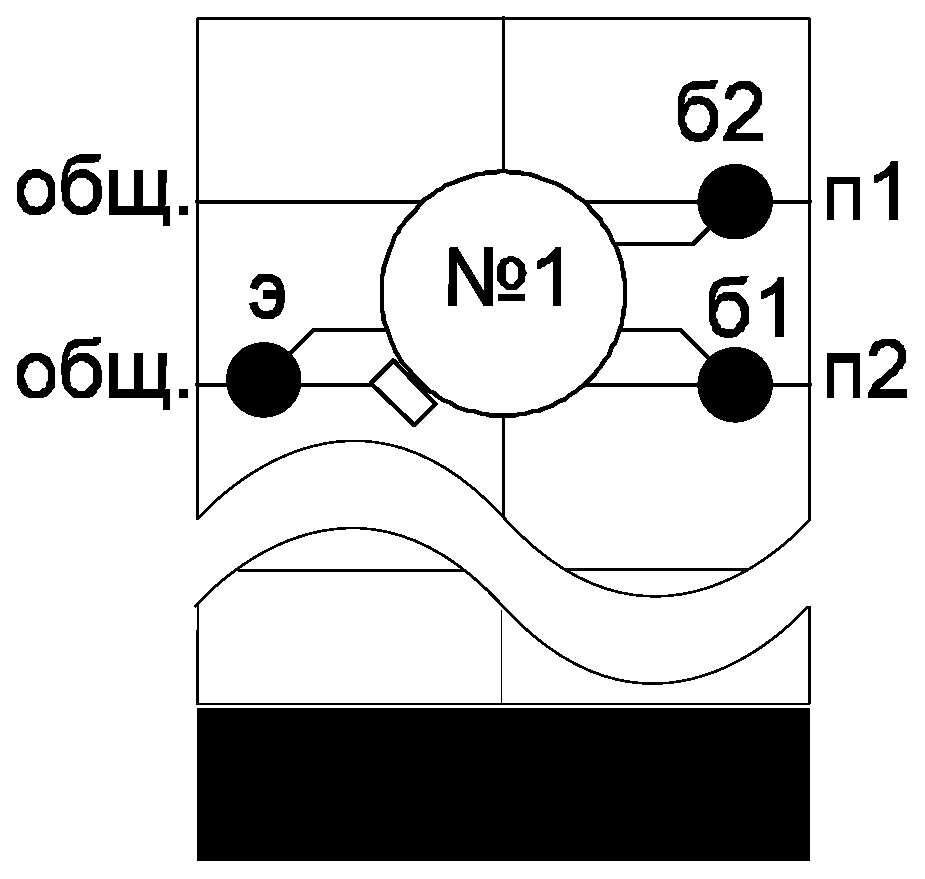
\includegraphics[width=0.6\linewidth]{pic1-install}
		\caption{Схема установки транзисторов в контактирующее
		приспособление. Транзисторы показаны выводами вниз.}
	\end{subfigure}
	\begin{subfigure}[t]{0.45\textwidth}
		\centering
		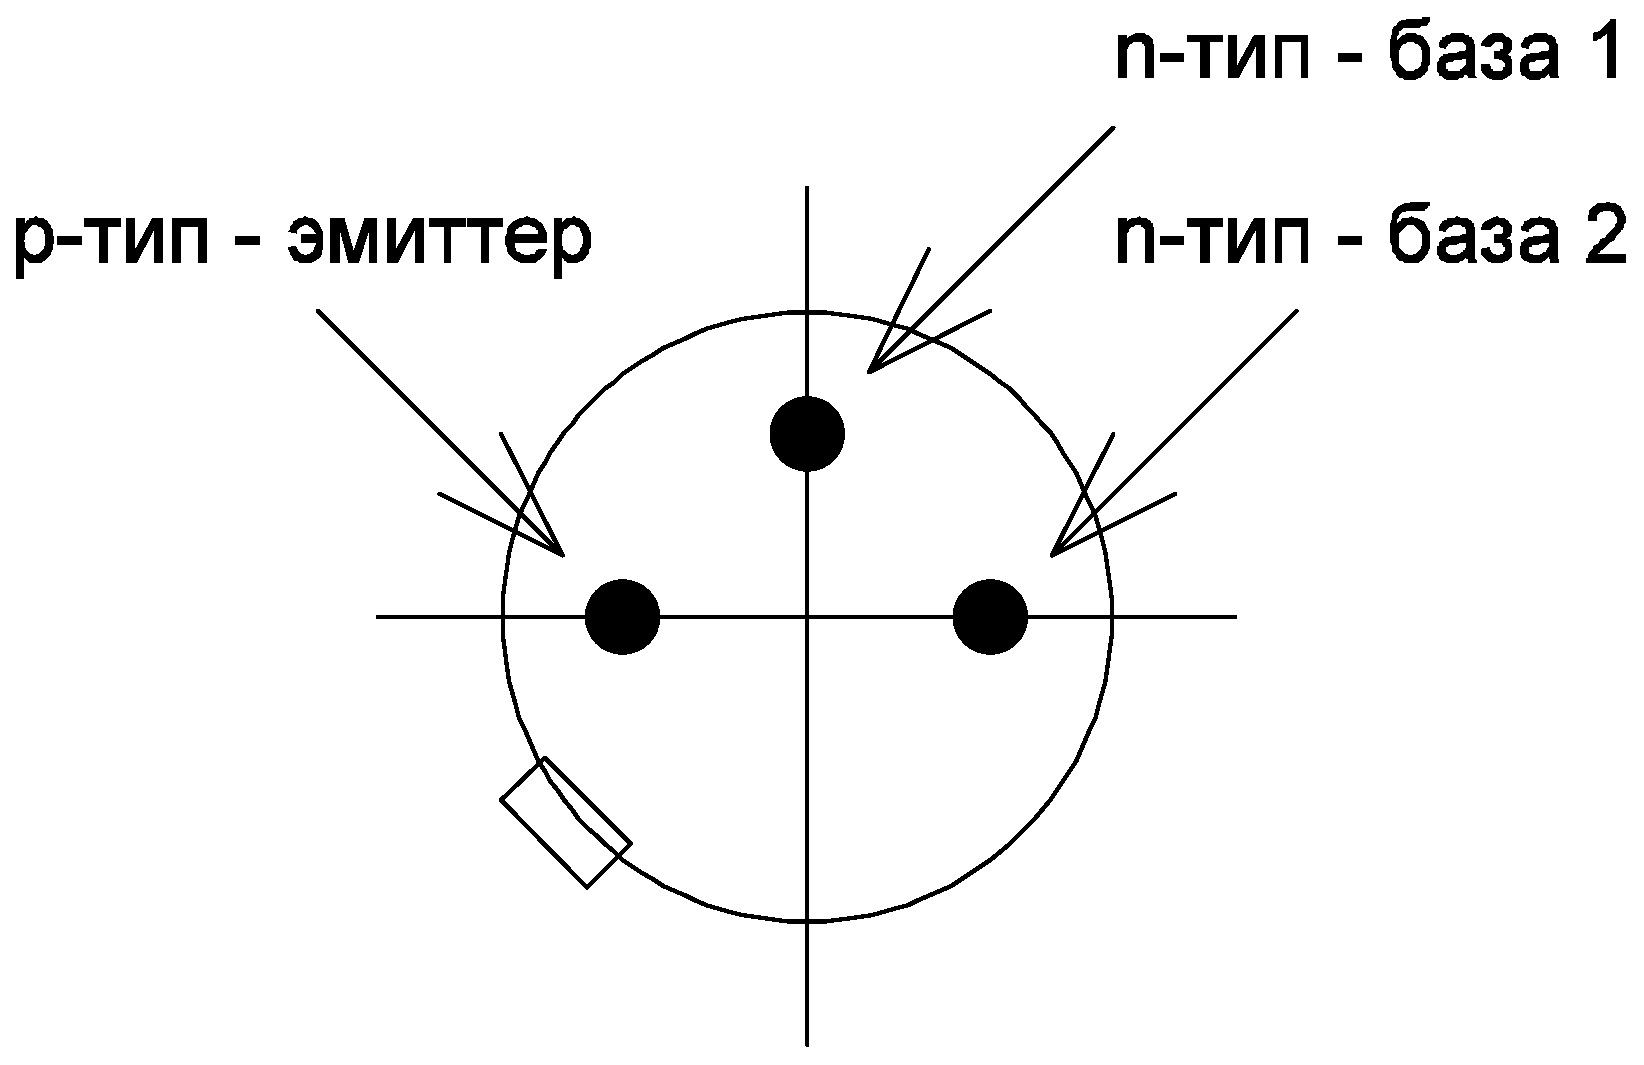
\includegraphics[width=0.9\linewidth]{pic1-pins}
		\caption{Расположение контактов транзистора КТ117Б. Транзистор
		показан выводами вверх.}
	\end{subfigure}

	\caption{Схема установки транзисторов.}
	\label{pic:installation}
\end{figure}

Условия, одинаковые для всех сканов перечислены в таблице 
\ref{table:common_conditions}.
\begin{table}[!ht]
	\centering
	\caption{Условия, одинаковые для всех сканов.}
	\begin{tabular}{|l|l|}
		\hline
		Параметр                           & Значение             \\ \hline
		Образцы                            & КТ117Б~№1            \\ \hline
		Длительность импульса, мкс         & 20                   \\ \hline
		Автоматическая компенсация моста   & включена             \\ \hline
		Шаг сканирования                   & 0.1                  \\ \hline
		Начальная частота сканирования, Гц & 1                    \\ \hline
		Конечная  частота сканирования, Гц & 2500                 \\ \hline
		Интервал между измерениями, с      & 3.5                  \\ \hline
		Постоянная интегрирования, с       & 3                    \\ \hline
	\end{tabular}
	\label{table:common_conditions}
\end{table}

На рисунке \ref{pic:p_coef_plot} показанны графики со значениями 
коэффициента $p$, соответствующих различным значениями разности $U_R - U_1$,
для трёх значений температуры образца: 263 К, 283 К, 303 К. На графиках 
отображены все пары $U_R$ и $U_1$ одновременно, что может частично 
обуславливать разброс.
\begin{figure}[!ht]
	\centering
	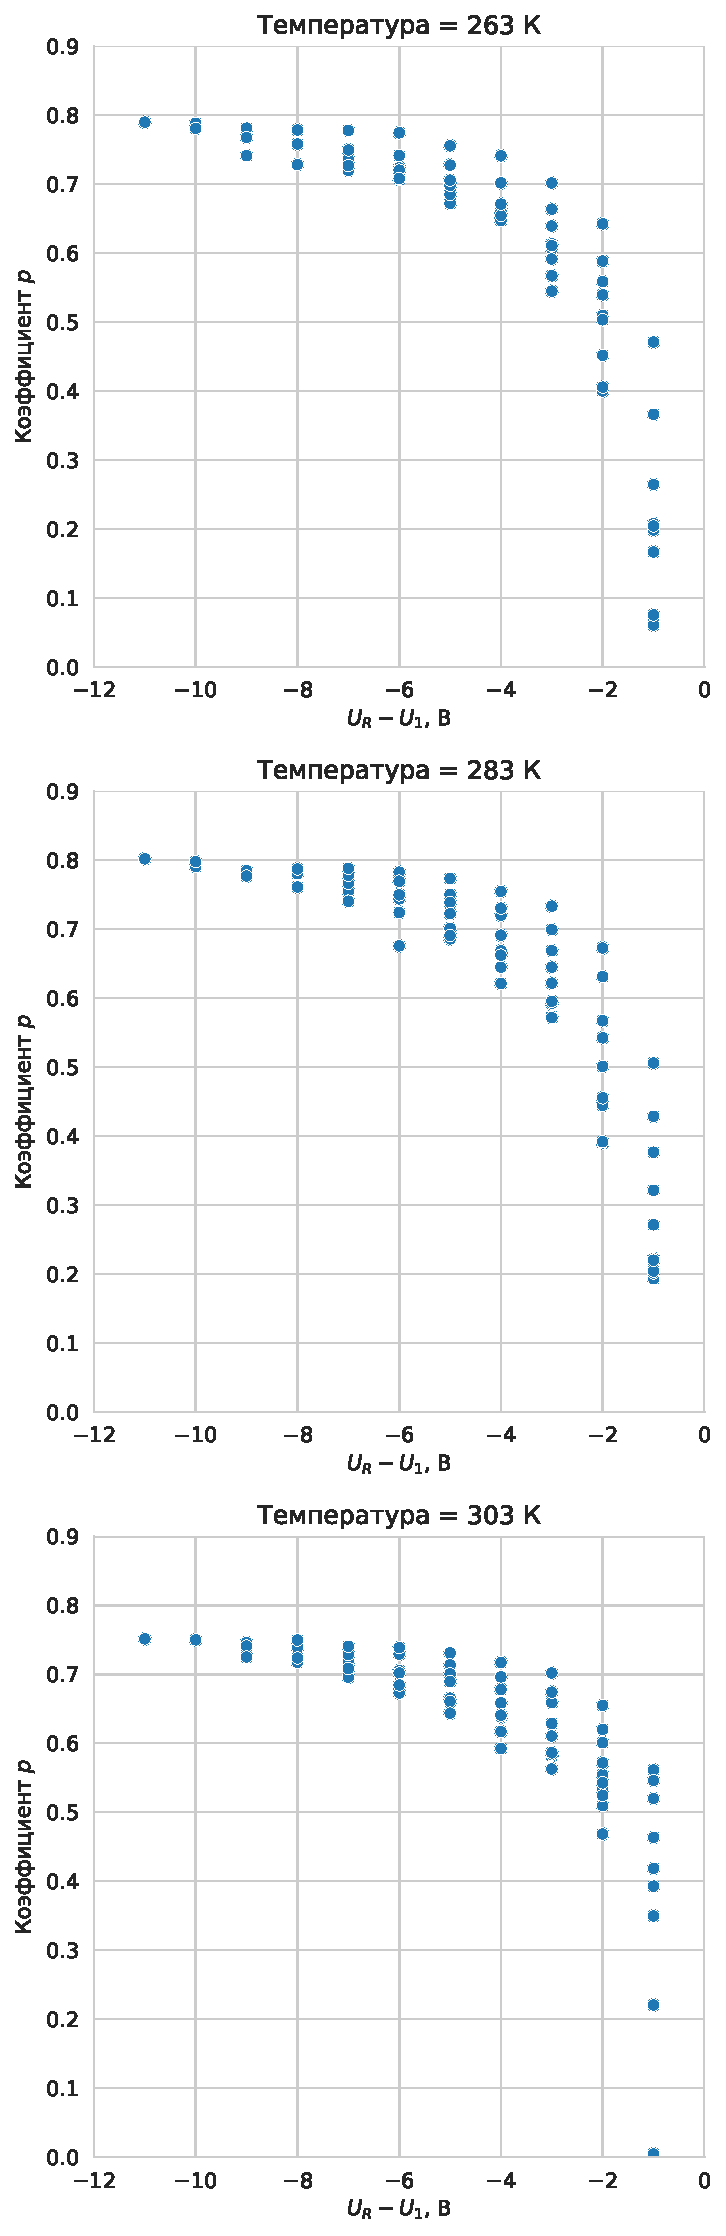
\includegraphics[height=0.95\textheight]{Зависимость_p_от_разности_u1_ur}
	\caption{Значения коэффициента $p$ для различных значений разности $U_R$ и $U_1$.}
	\label{pic:p_coef_plot}
\end{figure}